\chapter{Supersimetría}

\hll{Agregar introduccion}

\section{Problema de jerarquia}

El {\SM} de la física de altas energías descripto en el capítulo anterior,
con el agregado de la masa de los neutrinos, y el descubrimiento del bosón
de Higgs, ha tenido un gran éxito en la descripción de los fenómenos
conocidos hasta la escala del {\tev} a la que los experimentos han llegado
en los últimos a\~nos.
%% A pesar de esto, resulta claro que el Modelo Est\'andar no es una teoria definitiva y va a tener que
%% ser extendida para describir la f\'isica de altas energ\'ias.
A pesar de esto, no hay dudas respecto a que una nueva teor\'ia va a ser
necesaria a la escala reducida de Planck %% $M_P =  (8\pi G_\text{Newton})^{-1/2} = 2.4 \times 10^{18} \gev$ ,
donde los efectos cu\'anticos gravitacionales son importantes. Sabemos que
que tiene que existir nueva f\'isica en los 16 ordenes de magnitud en
energ\'ia entre el territorio explorado cerca de la escala electrod\'ebil
y la escala de Planck.
El s\'olo hecho de que la relación $M_P/M_W$ es tan grande es una gran pista
para la física mas allá del {\SM}, por el llamado \emph{problema de jerarquía}.
Este no es una dificultad intrínseca del {\SM}, sino una sensibilidad \hl{diusturbing}
del potencial de Higgs a nueva fisica en casi cualquier extension imaginable
del SM.
La parte eléctricamente neutra del campo de Higgs del SM es un escalar complejo
$H$ con un potencial clásico $V=m_H^2 |H|^2 + \lambda|H|^4$.
El SM necesita un valor de expectación del vacío (VEV) para $H$ en el
mínimo del potencial no nulo.
Esto ocurre si $\lambda>0$ y $m_H^2<0$, resultando en
$\avg{H} = \sqrt{-m_H^2/2\lambda}$.
Como experimentalmente sabemos que $\avg{H}$ es aproximadamente 174 \gev,
de las medidas de las propiedades de las interacciones débiles, el valor de
$m_H^2$ debe ser del orden de $-(100 \gev)^2$.

\begin{figure}[h]
  \centering
  \begin{tikzpicture}[node distance=1cm and 1 cm]

  \coordinate[vertex, label=above:$H$] (v1);
  \coordinate[vertex, right=of v1] (v2);
  \coordinate[vertex, right=of v2] (v3);
  \coordinate[vertex, right=of v3] (v4);

  \draw[higgs] (v1) -- (v2);
  \draw[higgs] (v3) -- (v4);

  \draw[fermion] (1.5, 0) circle (0.5);
  \node at (1.5, 0.75) {$f$};

\end{tikzpicture}

  \caption{Correciones cu\'anticas a un loop al cuadrado de la masa del Higgs
    $m_H^2$ debido a la masa de un fermi\'on de Dirac $f$.}
  \label{fig:higgs_correction_f}
\end{figure}

El problema es que $m_H^2$ recibe grandes correcciones cuánticas de los efectos
virtuales de cada partícula a la cual se acopla, directa o indirectamente, al
campo de Higgs. Por ejemplo, en la \cref{fig:higgs_correction_f} tenemos una
corrección a $m_H^2$ del loop que contiene un fermión de Dirac $f$ con masa
$m_f$. Si el campo de Higgs se acopla a $f$ con un término en el lagrangiano
igual a $-\lambda_f H \bar{f}f$, el diagrama de Feynman en la
\cref{fig:higgs_correction_f} genera una corrección:

\begin{equation}
  \Delta m_H^2 = -\frac{|\lambda_f|^2}{8\pi^2} \Lambda^2_\text{UV} + \ldots
  \label{eq:higgs_corr_f}
\end{equation}
%
donde $\Lambda_\text{UV}$ es el corte usado para regular la integral en el
\emph{loop}.
Debe ser interpretado como la m\'inima escala de energ\'ia a la cual entra
la nueva física para alterar el comportantamiento de la teoría a altas
energías. Los puntos suspensivos representan terminos proporcionales a
$m_f^2$, que crecen a lo sumo logaritmicamente con $\Lambda_\text{UV}$.
Cualquiera de los leptones o quarks del SM puede jugar el rol de $f$ (para
el caso de quarks la correcci\'on tiene que ser multiplicada por 3 para
tener en cuenta el color) y la correci\'on m\'as grande va a ser cuando
$f$ es el quark \emph{top} con $\lambda_f \approx 1$.

El problema aparece si $\Lambda_\text{UV}$ es del orden de $M_P$, ya que
la correci\'on a $m_H^2$ es 30 ordenes de magnitud mas grande que el valor
requerido de $m_H^2 \sim (100 \gev)^2$.
Este es sólo un problema para las correcciones al cuadrado de la masa del
bos\'on de Higgs escalar, porque las correcciones cuanticas a las masas de
los fermiones y los bosones de gauge no tienen una sensibilidad cuadratica
directa a $\Lambda_\text{UV}$ como la que estan en la \cref{eq:higgs_corr_f}.
Sin embargo, los quarks, leptones y los bosones de gauge electrodebiles
$Z^0$, $W^{\pm}$ del SM, todos obtienen masa de $\avg{H}$, por lo tanto el
espectro completo de masas del SM es directa o indirectamnte sensible a
la escala de corte $\Lambda_\text{UV}$.

Uno puede pensar que la soluci\'on es elegir un $\Lambda$ no demasiado
grande. Pero igual uno todavia deberia mezclar algo de neuva fisica
a la escala $\Lambda_\text{UV}$ que no solo altere los propagadores en
el loop, sino que corte la integral. Esto no es facil en una teoria cuyo
lagrangiano no conitene mas de dos derivadas, y las teorias de mayor orden
en derivadas generalmente sufren de fallas de unitariedad o causalidad.
%In string theories, loop integrals are nevertheless cut off at high Euclidean
%% momentum p by factors e −p /Λ UV . However, then Λ UV is a string scale that is usually † thought to be
%% not very far below M P . Furthermore, there are contributions similar to eq. (1.2) from the virtual effects
%% of any arbitrarily heavy particles that might exist, and these involve the masses of the heavy particles,
%% not just the cutoff.

\begin{figure}[h]
  \centering
  \begin{tikzpicture}[node distance=1cm and 1 cm]

  \coordinate[vertex, label=above:$H$] (v1);
  \coordinate[vertex, right=of v1] (v2);
  \coordinate[vertex, right=of v2] (v3);
  \coordinate[vertex, right=of v3] (v4);

  \draw[higgs] (v1) -- (v2);
  \draw[higgs] (v2) -- (v3);
  \draw[higgs] (v3) -- (v4);

  \draw[higgs] (1.5, 0.5) circle (0.5);

  \node at (1.5, 1.25) {$S$};

\end{tikzpicture}

  \caption{Correciones cu\'anticas a un loop al cuadrado de la masa del
    Higgs $m_H^2$ debido a la masa de un campo escalar $S$.}
  \label{fig:higgs_correction_s}
\end{figure}

En el caso de que exista un escalar complejo pesado $S$ con masa $m_S$
que se acopla al Higgs con un termino en el Lagrangiano
$-\lambda_S \abs{H}^2 \abs{S}^2$, el diagrama de Feynman es el que se
muestra en la \cref{fig:higgs_correction_s} y este da lugar a una
corrección:

\begin{equation}
  \Delta m_H^2 = \frac{\lambda_S^2}{16\pi^2} \left[ \Lambda^2_\text{UV} - 2 m_S^2 \ln (\Lambda^2_\text{UV}/m_S) +  \ldots \right]
  \label{eq:higgs_corr_s}
\end{equation}

%% Puede ser que el boson de Higgs no sea una fundamenta, como en modelos technicolor, o modelos en
%% los cuales el Higgs es compuesto.
Si el bosón de Higgs es una partícula fundamental y hay física a una
escala mucho mayor a la escala electrodébil, existen dos opciones:
tenemos que hacer alguna asumpcion bizarra que no existe ninguna
partícula de mayor masa o efectos que se acoplen (incluso indirectamente
o extremadamente débiles) con el campo escalar de Higgs, o algún tipo
de  cancelación es necesaria entre las varias contribuciones a $\Delta m_H^2$.

%------
% SUSY
%------
\section{Supersimetría}

La cancelación sistemática de las contribuciones a $\Delta m_H^2$ puede
ser realizada por una simetría. Comparando las \cref{eq:higgs_corr_f,eq:higgs_corr_s}
se puede ver que la nueva simetría tiene que relacionar bosones y fermiones,
debido al signo menos entre las contribuciones del loop fermionico y el
bosonico.

Afortunadamente la cancelación de todas estas contribuciones a las masas
escalares no solo es posible, sino que es inevitable, si consideramos
que existe una simetría que relaciona fermiones y bosones.
A esta simetría la llamamos supersimetría o SUSY.

Una transformación supersimétrica convierte un estado bosónico en uno
fermiónico, y viceversa. El operador $Q$ que genera estas transformaciones
debe ser un spinor anticonmutativo, con

\begin{equation}
  Q \ket{\text{bosón}} = \ket{\text{fermión}}, \quad \quad Q \ket{\text{fermión}} = \ket{\text{bosón}}
\end{equation}

Los espinores son intrínsecamente objectos complejos, por lo tanto el conjugado
hermitico de $Q$ es también un generador de la simetría. Debido a que $Q$ y $Q^\dagger$
son operadores fermiónicos, llevan momento angular de spin 1/2, por lo tanto es
claro que SUSY debe ser una simetria espacio-temporal y los operadores $Q$ y
$Q^\dagger$ deben satisfacer un algebra de la siguiente forma,

\begin{align}
  \{Q, Q^\dagger\} &= P^\mu \\
  \{Q, Q\} &= \{Q^\dagger, Q^\dagger\} = 0 \\
  [P^\mu, Q] &= [P^\mu, Q^\dagger] = 0 \\
\end{align}
%
donde $P^\mu$ es el cuadrimomento generador de las traslaciones espacio-temporales.

Los estados de partícula de una teoría supersimétrica son representados en
el álgebra de SUSY como \emph{supermultipletes}. Cada supermultiplete contiene
ambos estados, fermión y bosón, que son comúnmente llamados supercoma\~neros
uno de otro.

Los generadores $Q$ y $Q^\dagger$ conmutan con los generadores de las
transformaciones de gauge, por lo tanto las partículas en un mismo supermultiplete
tienen que estar en la misma representación del grupo de gauge, y tener la misma
carga eléctrica, isospin y color. El operador de masa $-P^2$ también conmuta con los
generadores y con todos los operadores de rotación y traslación, por lo tanto las
partículas que habiten el mismo supermultiplete deben tener los mismos autovalores
de $-P^2$, y entonces la misma masa.

Es fácil probar que cada supermultiplete tiene que contener igual numero de grados
de libertad fermiónico que bosónico, $n_B = n_F$.
La posibilidad mas simple para satisfacer esto es tener un único fermión de Weyl
($n_F=2$) y dos escalares reales (cada uno con $n_B=1$). Es natural poner estos
dos escalares en un único campo escalar complejo. Esta combinación de un fermión
de Weyl de dos componentes y un campo escalar complejo es llamado un supermultiplete
\emph{quiral} (o \emph{escalar} o de \emph{materia}).

Otra posibilidad es
que el supermultiplete contenga un bosón vectorial de spin 1. Para que la teoría
sea renormalizable, tiene que ser un bosón de gauge no masivo, al menos antes de
que la simetría de gauge sea espontáneamente rota. En este caso, este bosón contiene
dos estados de helicidad, $n_B=2$. Por lo tanto su supercomanero es un fermión de Weyl
de spin 1/2, con dos estados de helicidad, $n_F=2$. Si en vez de esto, uno intenta usar
un fermión de spin 3/2 la teoría no seria renormalizable. Los bosones de gauge deben
transformar como la represnetacion adjunta del grupo de gauge, por lo que sus compañeros
fermiónico, llamados \emph{gauginos}, también. Estas combinaciones de gauginos de
spin 1/2 y bosones de gauge de spin 1 es llamada supermultiplete de \emph{gauge} o
\emph{vectorial}.

Si incluimos la gravedad, el graviton de spin 2 (con dos estados de helicidad, $n_B=2$)
tiene un supercomanero de spin 3/2 llamado \emph{gravitino}.

Existen otras combinaciones posibles de particulaes que pueden satisfacer esta
condicion, pero siempre se reducen a combinaciones de supermultipletes quirales
de o de gauge, excepto en ciertas teorias con supersimetria extendida. Estas
teorias tuenbe mas de una copia de los generadores $Q, Q^\dagger$, pero no son
muy prometedoras desde el punto de vista fenomenologigo.
La teoria no extendida y fenologicamente viable es llamada generalmente $N=1$,
donde $N$ se refiere al numero de supersimetrias (el numero de las distintas
copias de $Q,Q^\dagger$).


%------
% MSSM
%------
\section{Modelo Mínimo Estándar Supersimétrico}

En una extensión supersimétrica del SM, cada una de las partículas fundamentales
conocidas esta contenida en un supermultiplete quiral o de gauge, y debe tener
un supercoma\~nero con spin que difiere en 1/2.
La extensión que requiere la introducci\'on de la minima cantidad de
partículas es llamado \emph{Modelo Mínimo Estándar Supersimétrico}, o MSSM.

%% The first step in understanding the exciting phenomenological consequences of
%% this prediction is to decide exactly how the known particles fit into supermultiplets, and to give them
%% appropriate names.

Solo los supermultipletes quirales pueden contener fermiones cuya parte izquierda
y derecha transforman de forma diferente bajo el grupo de gauge.
Todos los fermiones del SM (quarks y leptones) tienen esta propiedad,
por lo tanto deben ser miembros de supermultipletes quirales.
Los nombres de los compañeros de spin 0 de los quarks o leptones son construidos
anteponiendo una ``s'' (de \emhp{scalar}), y son llamados \emph{squarks}
y \emph{sleptones}, o \emph{sfermiones}.
La parte izquierda y derecha de los quarks y leptones son fermiones de Weyl
con diferentes propiedades de transformación de gauge del SM, entonces cada
uno debe tener un compañero escalar complejo.
Por ejemplo, los supercomañeros de la parte izquierda y derecha del campo
de Dirac de los electrones son llamadas parte izquierda y derecha de los
slectrones, {\selL} y {\selR}, aunque el subíndice no se refiere a la
helicidad de los slectrones (tiene spin 0) sino a la de sus supercomañeros.
Lo mismo ocurre para {\smuL}, {\smuR}, {\stauL} y {\stauR}. Los neutrinos
del SM son siempre izquierdos por lo que sus supercomañero se denotan:
{\snu}. Y para los quarks tenemos {\squarkL} y {\squarkR}, con $q = u, d, s, c, b, t$.
Las interacciones de gauge de cada uno de los campos de squarks y sleptones
son las mismas que la de los correspondientes fermiones del SM.

El bosón escalar de Higgs debe estar en un supermultiplete quiral ya que tiene
spin 0.
Dada la naturaleza de los campos quirales introducidos en la implementación de
SUSY, el campo escalar de Higgs no es suficiente para dar masa a los fermiones
de helicidad izquierda y derecha.
Se debe agregar un nuevo campo escalar para compensar. En el SM, el campo de
Higgs es un doblete, y de los cuatro grados de libertad solo uno permanece
como consecuencia del rompimiento de la simetría EW, resultando en un bosón
de Higgs. Los dos dobletes de Higgs del MSSM son:

\begin{equation}
  H_u = \binom{H_u^+}{H_u^0}, \quad \quad \quad H_d = \binom{H_d^0}{H_d^-}
\end{equation}

Los bosones vectoriales del SM tienen que estar en supermultipletes de gauge.
Sus super-compañeros fermiónicos son llamados \emph{gauginos}. Las interacciones
de gauge de color $SU(3)_C$ de QCD son mediadas por el gluon, cuyo compañero
supersimetrico de spin 1/2 es el \emph{gluino}. La simetría electrodébil
$SU(2)_L \times U(1)_Y$ esta asociada con los bosones de spin 1 $W^+, W^0, W^-$
y $B^0$, cuyos compañeros de spin 1/2 son $\susy{W}^+, \susy{W}^0, \susy{W}^-$
y $\susy{B}^0$, y llamados \emph{winos} y \emph{bino}.
Después de la ruptura de la simetría electrodébil, los auto-estados $W^0$ y $B^0$
se mezclan para dar $Z^0$ y $\gamma$. La correspondiente mezcla de {\winozero}
y {\bino} son llamados \emph{zino} (\zino) y \emph{fotino} (\photino).

La tabla....

\begin{figure}[h]
  \centering
  \includegraphics[width=0.9\textwidth]{figures/tabla}
\end{figure}

\section{Espacio de parámetros del MSSM}

Primero tenemos los parámetros usuales del SM: los acoplamientos
de gauge $g_s$, $g$ y $g'$, correspondientes al grupo de gauge
$SU(3) \times SU(2) \times U(1)$, respectivamente. Las constantes
de acoplamiento entre fermiones y Higgs: $\lambda_u$, $\lambda_d$
y $\lambda_e$ (correspondientes al acoplamiento de una generación
de quarks y leptones izquierdos y derechos, y sus supercompaneros,
a los bosones y Higgs y higgsinos). Otro parámetro es el parámetro de masa
del supercampo de Higgs $\mu$.

Los demás parámetros del MSSM aparecen
del los términos de rompimiento soft de SUSY. Estos incluyen tres
``gaugino Majorana mass parameters'' ($M_3, M_2$ y $M_1$),
diagonal squark and slepton mass squared-mass matrices in the $\susy{f}_L - \susy{f}_R$
($M^2_{\susy{Q}}$, $M^2_{\susy{U}}$, $M^2_{\susy{D}}$, $M^2_{\susy{L}}$ y $M^2_{\susy{E}}$),
Higgs-squark-squark and Higgs-slepton-slepton trilinear interaction terms
($A_t$, $A_b$ y $A_\tau$), y los parámetros de masa del sector de Higgs
($m^2_{1H}$, $m^2_{2H}$ y $m^2_{12}$).

 El rompimiento de la simetría electrodébil se realiza por los parámetros de masa
 de Higgs del rompimiento soft de SUSY. Como resultado de esto, $m^2_{1H}$, $m^2_{2H}$ y $m^2_{12}$
pueden expresarse en términos de dos valores de expectación del vacío ($v_1$ y $v_2$)
y una masa física de Higgs (en general se elige la masa del Higgs escalar CP-odd, $m_{A^0}$).
Como $v_1^2+v_2^2=(246 \gev)^2$ esta fijo por la masa del $W$ o $Z$, mientras que
el cociente $\tan \beta \equiv v_2/v_1$ es un parámetro libre del modelo.

En un modelo con una sola generación de quarks, leptones y sus supercomaneros,
la lista anterior tiene 14 nuevos parámetros. En el modelo completo de tres
generaciones, el numero de nuevos parámetros es sustancialmente mayor ya que
los parámetros de masa de los squarks y sleptones  y parámetros $A$ serán
matrices de $3 \times 3$, y la posibilidad de mezcla entre generaciones puede
llevar a complicaciones adicionales. Sin embargo, no todos estos parámetros
son físicos. Algunos de estos parámetros pueden ser eliminados expresando
los auto-estados de interacción en términos de los auto-estados de masa, con la
apropiada redefinicion de los campos del MSSM para remover los grados de
libertad no físicos. El análisis de la \hl{ereferencia 55(S. Dimopoulos and D. Sutter, Nucl. Phys. B452, 496}
(1995);) muestra que el MSSM posee 124 parámetros independientes.
De estos, 18 corresponden a los parámetros del SM, uno corresponde
al sector de Higgs (el análogo a la masa del Higgs del SM), y 105 son
nuevos parámetros del modelo.

Realizar predicciones y análisis fenomenológicos con 14 o mas parámetros
es impracticable. Es por este motivo, que para esto se hacen suposiciones
para reducir la libertad de parámetros. Es por esto que hay que no existe
una definición precisa del MSSM. Es importante conocer cuales son las suposiciones
que se han hecho.

En un tratamiento fenomenológico completo todos los parámetros del MSSM
debería dejarse libres y deberían determinarse a partir de los datos. Una
vez que los parámetros sean medidos, uno puede intentar extraer información de
la física subyacente que esta asociada con escalas de energía a la probada en
colosionadores. Ya que la conjetura principal de SUSY esta motivada por el
intento de embed la física de bajas energías en un modelo mas fundamental, es
apropiado explotar esta motivación en contraining los parámetros de SUSY a
bajas energías.


\subsection{El espectro de masas del MSSM}

Una característica importante del MSSM es que las súper-compañeras listadas en la
tabla no son necesariamente autoestados de masa de la teoría. Esto es porque después
del rompimiento de la simetría electrodébil y de SUSY, puede haber mezcla entre
los gauginos y higgsinos, y entre los squarks y sleptones y los Higgs escalares
que tienen la misma carga eléctrica. La única excepción es el gluino.

En el MSSM, la descripción del rompimiento de la simetría electrodéebil es un
poco mas complicada debido al hecho de que hay dos dobletes complejos de Higgs
$H_u$ y $H_d$ en vez de solo uno como en el SM.

\note{explicar minimamente el rompimiento}

%% En el MSSM los higgsinos neutros y los gauginos se mezclan para formar los cuatro neutralinos:
%% \ninoone, \ninotwo, \ninothree\ y \ninofour.
%% Y de forma similar los higgsinos cargados y los winos dan lugar a los dos charginos, \chinoonepm\ y \chinotwopm.


%% con un total de 8 grados de libertad, 3 de los cuales se pierden en el rompimiento
%% de la simetria EW. Por lo tanto quedan 5 bosones de Higgs en el MSSM: $h^0, H^0, H^+, H^-, A^0$.
%% El más liviano de los 5 es $h^0$, el cual es el más similar al del SM.


%%\subsection{Neutralinos y Charginos}

Los higgsinos y los gauginos electrodebiles se mezclan entre ellos debido al\note{arreglar}
efecto del rompimiento de la simetría electrodébil. Los higgsinos neutros
($\susy{H}_u^0$ y $\susy{H}_d^0$) y los gauginos neutros (\bino, \winozero)
se combinan para formar cuatro autoestados de masa llamados neutralinos.
Los higgsinos cargados ($\susy{H}_u^+$ y $\susy{H}_d^-$) y los winos
(\winop y \winom) se mezclan para formar dos autoestados de masa con carga
$\pm 1$ llamados charginos.
En general se suele utilizar la siguiente notación para llamar a los
neutralinos y charginos:
${\nino}_{i}$ ($i=1,2,3,4$) y ${\chinopm}_{i}$ ($i=1,2$) donde estos son
ordenados de forma ascendente según su masa. El neutralino mas liviano
{\ninoone}, suele ser la LSP, salvo que exista un {\gravino} más liviano
o que la paridad-R no se conserve.

La mezcla de los gauginos cargados (\winopm) y los higgsinos
cargados ($H_u^+$ y $H_d^-$) esta descripta a orden arbol por
la matriz de 2 x 2:

\begin{equation}
  M_{C} = \left(
  \begin{array}{cc}
    \M{2} & \frac{1}{\sqrt{2}} g v_u \\
    \frac{1}{\sqrt{2}} g v_d & \mu \\
  \end{array}
  \right)
\end{equation}

y para determinar los estados fisicos y las masas de los
charginos hay que diagonlizarla.
%% Los estados fisicos $\chinoonepm$
%% y {\chinotwopm}


En la base de autoestados de gauge $\psi^0 = (\bino, \winozero, \susy{H_d^0}, \susy{H}_u^0)$,
la parte de masa del neutralino del Lagrangiano es

\begin{equation}
  \mathcal{L}_\text{neutralino mass} = -\frac{1}{2} (\psi^0)^T M_{\nino} \psi^0 + c.c.
\end{equation}
%
donde

\begin{equation}
  M_{\nino} = \left(
  \begin{array}{cccc}
    \M{1} & 0 & -c_\beta s_W m_Z &  s_\beta s_W m_Z \\
    0 & \M{2} & c_\beta c_W m_Z & -s_\beta c_W m_Z \\

    -c_\beta s_W m_Z & c_\beta c_W m_Z & 0 & -\mu \\
    s_\beta s_W m_Z & -s_\beta c_W m_Z & -\mu & 0 \\
  \end{array}
  \right)
\end{equation}

Esta matriz de masas puede ser diagonalizada con una matriz unitaria $N$ para obetener los autoestados
de masa:

\begin{equation}
  \nino_i = N_{ij} \psi^0_j
\end{equation}

Los autoestados de masas y la matriz de mezcla $N_{ij}$ pueden obtenerse en termino de los parámetros
\M{1}, \M{2}, $\mu$ y $\tan\beta$.

El sector de los neutralinos esta determinado por tres parámetros reales, \M{1}, $\tan\beta$ y
$\mu$ (como también por supuesto $m_Z$ y $\theta_W$).

El espectro de masa de los charginos puede analizarse de forma similar.

Como el gluino es un \fix{colour octet fermion}, no puede mezclarse con ninguna
otra partícula del MSSM, incluso si la paridad-R es violada.
%% La mayoría de los
%% modelos asumen que la masa del gluino es significativamente mayor  que los
%% %% neutralinos y charginos.


%% \hll{Falta squarks, sleptons}

Si un estado de chargino o neutralino se aproxima a un estado
particular de gaugino o higgsino, es conveniente usar la nomenclatura
correspondiente. Si \M{1} y \M{2} son pequenas comparadas a $m_Z$ y $|\mu|$,
el neutralino mas liviano va a ser puramente fotino. Si \M{1} y $m_Z$ son pequenos comparados
a \M{2} y $|\mu|$, entonces el neutralino mas liviano va a ser puramente bino.
Si \M{2} y $m_Z$ son pequenas comparadas con \M{1} y $|\mu|$, el par de charginos mas liviano y
neutralino va a constituir un triplete de winos puro degenerado en masas.
Finalmente, si $|\mu|$ y $m_Z$ son chicos comparados con \M{1} y \M{2},
el neutralino mas liviano va a ser un higgsino puro. Cada unos de los
casos anteriores va a llevar a un fenomenologia muy distinta.


\subsection{Decaimiento de spartículas}

\subsubsection{Neutralinos y charginos}

Como cada neutralino y chargino contiene al menos una mezcla
de los gauginos electrodebiles {\bino}, $\tilde W^0$ o $\susy{W}^{\pm}$
, heredan los acoplamnientos de strength electrodebil a los pares
de fermiones escalaes. Si los sleptones o squarks son lo sufientemente
livianos, un neutralino o chargino va a decar a un par lepton+slepton
o quark+squark. Tambien pueden decaer en un neutralino o chargino
mas liviano mas un Higgs escalar o un boson de gauge electrodebil.
Los posibles decaimientos son

\begin{align*}
  &\susy{N}_i \to Z \susy{N}_j, \quad W \susy{C}_j, \quad h^0 \susy{N}_j, \quad \ell \susy{\ell}, \quad \nu \susy{\nu}, \quad
  [A^0 \susy{N}_j, \quad H^0 \susy{N}_j, \quad H^{\pm} \susy{C}_j^{\mp}, \quad q \susy{q}], \\
  &\susy{C}_i \to W \susy{N}_j, \quad Z \susy{C}_1, \quad h^0 \susy{C}_1, \quad \ell \susy{\nu}, \quad \nu \susy{\ell}, \quad
  [A^0 \susy{C}_1, \quad H^0 \susy{C}_1, \quad H^{\pm} \susy{N}_j, \quad q \susy{q}']
\end{align*}
%
donde los estados finales entre corchetes son los cinematicamente menos probables.

\subsubsection{Sleptones}

Los sleptones puede decaer en un lepton y un chargino o neutrlaino,

\begin{align}
  \slepton &\to \ell \nino, \nu\chinopm \\
  \snu &\to \nu\nino, \ell\chinopm
\end{align}

Como los sleptones derechos no se acoplan al gaugino de $SU(2)_L$,
comunmente prefieren el decaimiento directo a $\ell\ninoone$.

\subsubsection{Gluino}

El gluino solo puede decaer a traves de un squark, ya sea on-shell o
virtual. Si el decaimiento a dos cuerpos esta abierto, este va a
dominar debido al acoplamiento gluin-quark-squark tiene intensidad QCD.
En el caso de que todos los squarks sean mas pesados que el gluino,
este va a decaer solo squarks virtuales.

\begin{align}
  &\gluino \to q\susy{q}, \\
  &\gluino \to qq\nino, qq^\prime \chinopm
\end{align}


\subsubsection{Squarks}

Los squarks puede tener decaimiento a dos cuerpos en un squark-gluino
si esta cinematicamente permitido, porque tiene QCD strength. Por otro
lado, los squarks pueden decaer en un quark y un neutralino/chargino.

\begin{equation}
  \susy{q} \to q\gluino, q\nino, q^\prime \chinopm
\end{equation}

%% El gluino, chargino o neutralino que resulta del decaimiento de un squark
%% va a decaer
%% The gluino, chargino or neutralino resulting from the squark decay will in turn
%% decay, and so on, until a final state containing χ  ̃ 1 is reached. This results in
%% numerous and complicated decay chain possibilities called cascade decays.


\subsection{Paridad R}

La forma general del superpotencial del MSSM tiene como inconveniente que
el numero leptonico y barionico no es una cantidad conservada. Esto
implica que el protón puede decaer a través del intercambio del compañero
escalar del quark down. Esto se contradice claramente con el limite superior
medido en la vida media del protón, que es $> 10^{30}$ a\~nos a $90\%$ CL\cite{PDG}.

Para evitar este problema, la estrategia mas comúnmente utilizada es introducir
una nueva simetría. Esta simetría se la conoce como paridad-R y puede escribirse como,

\begin{equation}
  P_R = (-1)^{3(B-L)+ 2s}
\end{equation}
%
donde $B$ y $L$ son respectivamente el numero barionico y leptonico, y $S$ es
el spin de la particula. Las partículas con paridad-R impar se llaman partículas
supersimétricas o \emph{spartículas}, mientras que las particulas del SM tiene
$P_R = +1$.

Si la paridad-R es exactamente conservada, no puede haber mezcla entre
las spartículas y las particulas con $P_R = +1$. Cada vertice de interacción
en la teoría contine un número par de spartículas.
Esto tiene tres consecuencias fenomenológicas de extrema importancia:

\begin{itemize}
\item La partícula supersimétrica mas liviana, llamada LSP, debe ser estable. Si la LSP es
  electricamente neutra, interactua solo de forma débil con la materia ordinaria, y por lo tanto
  resulta en un candidato muy atractivo para la materia oscura no barionica que es requerida por
  la cosmología.
\item Cada partícula supersimétrica que no sea la LSP debe decaer eventualmente en un estado que
  contenga un número impar de LSPs (en general una).
\item En experimentos de colisionadores, las partículas supersimétricas pueden sólo ser producidas
  en número par, en general de a dos.
\end{itemize}


%% where B and L are respectively baryon and lepton number and S is the spin of a particle.
%% R-parity is a discrete multiplicative symmetry, that must be conserved in all interactions. For
%% all the particles of the Standard Model the eigenvalue of R = 1 and for all their superpartners
%% R = −1. This has profound experimental consequences:
%% • Being a multiplicative symmetry the number of SUSY particles in any given interaction is
%% always conserved modulo two. Hence supersymmetric particles can only be produced in
%% pairs from Standard Model particles.
%% • At the LHC SUSY particles with strong interaction couplings will have highest production
%% rates. A coloured supersymmetric particle will decay in a chain until the lightest SUSY
%% particle is produced. These cascade decays have as signature multiple high momentum
%% jets and possibly leptons.
%% • The Lightest Supersymmetric Particle (LSP) is absolutely stable as it has no particle with
%% R = −1 to decay to. A clear signature from SUSY particle decay is the large missing
%% energy that is carried away by the LSP.
%% The LSP is considered a good candidate for the dark matter content of the universe.








%---------------------
% Rompimiento de SUSY
%---------------------
\section{Rompimiento de la Supersimetría}

Los supermultipletes quirales y de gauge de la tabla XXX conforman el contenido
de partículas del MSSM. Desde el punto de vista experimental, ninguna de las
compa\~neras supersimétricas de las partículas del SM han sido observadas hasta
el momento.
Si la supersimetr'ia no estuviera rota, deberían existir selectrones con una masa igual
a $m_e \sim 0.511 \mev$, y lo mismo para los demás sleptones y squarks. Y también
deberían existir los gluinos y fotinos sin masa.
El hecho de que no hayan sido descubiertas hasta el momento es motivo evidente
de que SUSY es una simetría que esta rota en el estado de vacío elegido
por la naturaleza.

Pero una de las principales motivaciones para introducir esta nueva simetria
fue que las divergencias cuadráticas en el cuadrado de las masas escalares
podian anularse a todo orden en teoría de perturbaciones, y esto esta garantizado
solo si esta simetria no esta rota.
Para que SUSY todavía pueda proveer la solución al problema de jerarquía incluso
en presencia del rompimiento de esta, las relaciones entre los acoplamientos
adimensionales que están en la teoría no rota deben mantenerse.
Para que esto suceda, el rompimiento de la supersimetría debe ser \emph{soft}.
El Lagrangiano efectivo del MSSM tiene que poder ser escrito como:

\begin{equation}
  \mathcal{L} = \mathcal{L}_\text{SUSY} + \mathcal{L}_\text{soft}
\end{equation}
%
donde $\mathcal{L}_\text{SUSY}$ contiene todas las interacciones de gauge y
de Yukawa y preserva la invarianza supersimétricas, y $\mathcal{L}_\text{soft}$
viola supersimetría pero contiene solo términos de masa y parámetros de
acoplamientos con dimensión de masa positiva.
Si la escala de masa mas grande asociada  con los términos soft se llama $m_\text{soft}$,
las correcciones adicionales no supersimétricas al cuadrado de la masa escalar del Higgs
debe anularse en el limite $m_\text{soft} \to 0$.

Debido a que la diferencia de masas entre las partículas conocidas del SM y sus
súper compañeras son determinadas por los parámetros $m_\text{soft}$ que aparecen
en $\mathcal{L}_\text{soft}$, las masas de las partículas supersimétricas no
pueden ser demasiado grandes. De otra forma perderíamos la solución al problema
de jerarquía.

Por otro lado, también existe una razón por la cual las partículas supersimétricas
deben ser lo suficientemente pesadas para no haber sido descubiertas hasta ahora.
Todas las demás partículas del MSSM que han sido observadas tienen algo en común:
deberían no tener masa en ausencia del rompimiento de la simetría electrodébil.
En particular, las masas de los bosones $W^\pm$, $Z^0$ y todos los quarks y
leptones son iguales a constantes de acoplamiento adimensionales por el
$\avg{H} \sim 174 \gev$, mientras que el fotón y el gluon necesitan ser no masivos
por la invarianza de gauge electromagnética y de QCD. Por el contrario, todas
las partículas del MSSM no descubiertas tienen la propiedad contraria. Cada una
de ellas pueden tener un término de masa en el Lagrangiano en ausencia del
rompimiento de simetría electrodébil.

En el MSSM, el rompimiento de SUSY es introducido explícitamente.
El rompimiento de una simetría global siempre implica un modo
no masivo de Nambu-Goldstone con los mismos números cuánticos que
el generador de la simetría rota. En el caso de la supersimetría
global, el generador es la carga fermionica $Q_\alpha$, por lo
tanto la partícula de Numbu-Goldstone tiene que se un formón
de Weyl no masivo neutro, llamado \emph{goldstino}.
Es claro ahora que el rompimiento espontáneo de la supersimetría
requiere la extensión del MSSM.
El rompimiento espontáneo de SUSY tiene que ocurrir en un
<<sector oculto>>  de partículas que no tienen acoplamientos
directos con los supermultipletes quirales (<<sector visible>>)
del MSSM. Sin embargo, estos dos sectores comparten algunas
interacciones que son las responsables de mediar el rompimiento
de la supersimetría desde el sector oculto al visible, resultando
en los términos soft del MSSM (ver figura).

\begin{figure}[h]
  \centering
  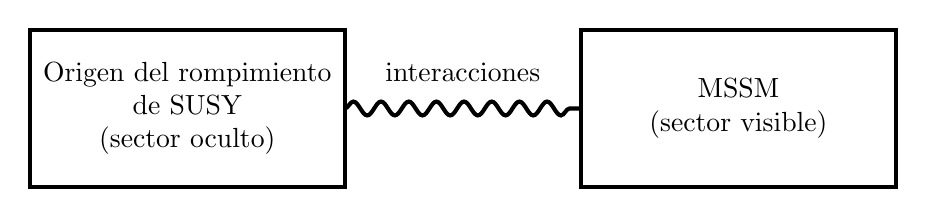
\begin{tikzpicture}

  \draw[line width=1.5] (0,0) rectangle (4,2) node[midway,align=center] (r1) {Origen del rompimiento\\ de SUSY\\ (sector oculto)};
  \draw[line width=1.5] (7,0) rectangle (11,2) node[midway, align=center] (r2) {MSSM\\ (sector visible)} ;

  \draw[line width=1.5,decorate,decoration={snake}] (4,1) -- (7,1) node[midway,above=.2cm] {interacciones};

\end{tikzpicture}

\end{figure}

Existen muchas propuestas de como estas interacciones
mediadores puede ser. Una de estas (e historicamnete la mas popular)
es que estas interacciones son gravitacionales (SUGRA). Mas precisamente
estas asociados con la nueva física, incluyendo a la gravedad, que
aparece cerca de la escala de Planck. En este escenario

Una segunda posibilidad es que estas interacciones mediadores sean
as interacciones de gauge electrodébil y QCD ordinarias. En estos
escenarios donde el rompimiento de supersimetría esta mediado por
campos de gauge (GMSB), los términos soft del MSSM provienen de
diagramas a un loop que involucran algunas partículas mensajeras.

Si tenemos en cuenta a la gravedad, la supersimetría tiene que ser
promovida a una simetría local. Esta teoría supersimétrica local
es llamada \emph{supergravedad}. Esto unifica necesariamente las
simetrías espacio-temporales ordinarias de la Relatividad General
con las transformaciones locales supersimétricas. En esta teoria,
el graviton de spin 2, tiene un supercompa\~nero fermión de spin 3/2
llamado \emph{gravitino}. Mientras la supersimetría no este rota,
el graviton y el gravitino son no masivos con dos estados de helicidad
de spin. Una vez que SUSY es espontáneamente rota, el gravitino adquiere
una masa absorbiendo el goldstino, que se convierte en sus componentes
longitudinales (helicidad $\pm 1/2$). Este mecanismo es llamado \emph{super-Higgs},
y es el análogo al mecanismo de Higgs ordinario de las teorías de gauge,
donde los bosones de gauge $W^\pm$ y $Z^0$ en el {\SM} adquieren
masa absorbiendo los bosones de Nambu-Goldstone asociados con la
invarianza de gauge electrodébil espontáneamente rota. La masa del
gravitino es tradicionalmente llamada $m_{3/2}$, y puede ser estimada
como

\begin{equation}
  m_{3/2} \sim \avg{F} / M_P
\end{equation}

Esto implica distintos valores esperados para la masa del gravitino
dependiendo el modelo de mediadores propuesto. En modelos de mediación
por gravedad, la masa del gravitino es comparable a la masa de las
sparticulas del MSSM, por lo tanto es esperado que sea de al menos
el orden de 100 \gev. Sus interacciones van a ser de intensidad
gravitacional, el gravitino no juega ningún rol en física de
colisiona dores, pero puede ser importante en cosmología.

En contraste, los modelos GMSB predicen un gravitino mucho mas
liviano que las sparticulas del MSSM si $M_\text{mess} \ll M_P$.
En este caso, el gravitino es la LSP, y todas las sparticulas
del MSSM van a decaer eventualmente en un estado final que incluye
el gravitino.








%------
% GMSB
%------
\section{GMSB} %%Modelos de rompimiento de supersimetría mediados por campos de Gauge}

En los modelos de rompimiento de la supersimetría mediado por campos de gauge
(GMSB), las interacciones ordinarias de gauge son los responsables de la
aparición del rompimiento de la supersimetría \emph{soft} en el MSSM.
La idea básica es introducir
nuevos supermultipletes quirales, llamados mensajeros, que se acoplen ...
\note{Referencia: arxiv:9801271}

Estos modelos ofrecen una rica variedad de signaturas en colisionadores\note{0911.4130}.
La caracteristica mas destacable de estos modelos es el gravitino liviano
$m_{3/2} = M_\text{weak}$. Esto asegura que los efectos de mediacion por
campos de gauge domine por sobre la mediacion por gravedad. Esto implica
que la particula mas liviana del MSSM es la NLSP, que siempre decaera
en un gravitino y un companero del SM.
El gravitino siempre va a escapar del detector, dejando una cantidad
significativa de energia faltante. Mientras tanto, el companero del SM va
a tender a ser central y energetico (asumiendo que la NLSP decae promptly),
ya que es en general mucho mas liviano que la NLSP. Dado que en cada evento
SUSY se producen dos NLSPs, es claro que las signaturas en un colisionador
van a estar determinadas por la naturaleza de la NLSP.


In gauge-mediated supersymmetry breaking, gauge forces
transmit the supersymmetry breaking to the MSSM. A typical
structure of such models involves a hidden sector where supersymmetry
is broken, a messenger sector consisting of particles
(messengers) with SU(3)×SU(2)×U(1) quantum numbers, and
the visible sector consisting of the fields of the MSSM [38–40].
The direct coupling of the messengers to the hidden sector generates
a supersymmetry-breaking spectrum in the messenger
sector. Finally, supersymmetry breaking is transmitted to the
MSSM via the virtual exchange of the messengers. In models
of direct gauge mediation, the supersymmetry-breaking sector
includes fields that carry Standard Model quantum numbers, in
which case no separate messenger sector is required [41].

The gravitino mass in models of gauge-mediated supersymmetry
breaking is typically in the eV range (although in some
cases it can be as large as a GeV), which implies that Ge is
the LSP. In particular, the gravitino is a potential dark matter
candidate (for a recent review and guide to the literature, see
Ref. 17). The couplings of the helicity ±1/2 components of Ge
to the particles of the MSSM (which approximate those of
the goldstino, cf. Section I.2.3) are significantly stronger than
gravitational strength and amenable to experimental collider
analyses



\subsection{La LSP: El gravitino}

Como resultado del rompimiento espontaneo de la supersimetria, el espectro fisico
contiene un fermion no masivo de spin 1/2, el goldstino. Cuando la teoria supersimetrica
global esta acoplada a la gravedad y promocionada a una teoria supersimetrica local,
el goldstino provee los modos longitudinales de spin 3/2 del graviton: el gravitino.
Como resultado de este mecanismo de super-Higgs, el gravitino adquiere una masa
que bajo la condicion de la anulacion de la constante cosmologica esta dada por:

\begin{equation}
  m_{3/2} = \frac{F_0}{\sqrt{3}M_P}
\end{equation}
%
donde $M_P = (8\pi G_N)^{-1/2} = 2.4 \times 10^{18} \gev$ es la masa reducida de Planck.
Y $F_0$ es la contribucion total del VEV de rompimiento de SUSY de los campos auxiliares
normalizado de tal forma que la energia de vacio de la teoria supersimetrica global es
$V = F_0^2$...

En los modelos GMSB, el gravitino es la particula supersimetrica mas liviana (LSP) para
cualquier valor relevante de $F$. Si la paridad-R es conservada, todas las particulas
supersimetricas van a seguir cadenas de decaimineto que terminan en gravitinos.

%% Para
%% calcular la tasa de decaimiento
%% La caracteristica mas representativa de los modelos GMSB es el gravitino liviano

\subsection{La NLSP}

\hl{La NLSP puede ser cualquier .... Focus on neutralino NLSP}

La segunda particula supersimétrica mas liviana (NLSP) juega un rol
fundamental en la fenomenología de los modelos GMSB. Asumiendo que se
conserva la paridad-R, todas las particulas supersimétricas van a decaer
rapidamente en una cascada hasta la NLSP, y esta va a decaer en un gravitino
via interacciones 1/F. Por este motivo, la naturaleza de la NLSP
determina las signaturas en los colisionadores y algunas propiedades
cosmologicas del GGM. La NLSP puede ser, dependiendo de la eleccion \note{ref a http://arxiv.org/pdf/hep-ph/9801271v2.pdf}
de los parametros, el neutralino, el stau, y en algunas regiones del
espacio de parametros muy restrictivas, el sneutrino.

En el caso de que sea neutralino, esta tiene, en la mayoria de los
casos, una componente dominante de bino, ya que el cociente $\mu/\M{1}$
es generalemente mayor a 1. %Una excepcion ocurre para N grande y M y lambda
%chico?

Las tazas de decaimiento del {\ninoone} NLSP son:\note{pongo las formulas?}

\begin{align}
  \Gamma (\ninoone \to \gamma \gravino) =
\end{align}

Las particulas, que aunque no son NLSP, tienen un decaimiento dominante en
su companero supersimetrico y el {\gravino} se denominan \emph{co-NLSP}.
Para valores grandes de $\tan \beta$, las dos primeras generaciones de
sleptones decaen como $\susy{\ell}_R \to \ell \tau \stau$ y el stau
es la ``unica'' NLSP. Otra posibilidad es que el {\ninoone}, aunque no sea
la NLSP, esta degenerado en masa con el {\stau}, y su decaimiento dominante
sea a un foton y un goldstino. En este caso {\stau} y {\ninoone} son co-NLSP.

La posibilidad de que el sneutrino sea NLP es muy marginal. Requiere valores
de $N$ tan grandes y valores tan chicos de $\Lambda$ que el descubrimiento de
SUSY deberia darse muy pronto. En este caso el sneutrino decae en un neutrino
y un goldstino.

Todos estos casos corresponden a una fenomenologia completamente diferente en
los experimentos de altas energias.

\subsection{Neutralino NLSP}

En el caso de que la NLSP sea el neutralino, la fenomenología se puede entender
mejor yendo a algunos limites simplificados de los autoestados. De esta forma
los distintos tipos son:

\begin{itemize}
\item bino NLSP
\item wino co-NLSP
\item higgsino NLSP
\end{itemize}

%% We will formulate minimal spectra in this paper which allow for significant strong SUSY production at the early LHC,
%% and populate the many final states   available to general neutralino NLSPs.

%% El espacio de parámetros consiste esencialmente en una escala de producción de color (masa del gluino)
%% y la masa de la NLSP. Todas las demás sparticulas se desacoplan que no son esecnailes en la producción
%% de la signatura de interés. De alguna forma, esto es similar a utilizar ``modelos simplificados'' como
%% se utilizan en muchos estudios fenomenológicos y experimentales. \todo{add references?}

El neutralino NLSP decae a $X + \gravino$, donde $X=\gamma, Z, h$, y los
diferentes autoestados de gauge se caracterizan por tener distintos
BR a las diferentes $X$.

  %% The branching fractions of the bino-like and wino-like neutralino NLSP are shown in the figure.
  %% \includegraphics[width=0.5\textwidth]{br_bino}
  %% \includegraphics[width=0.5\textwidth]{br_wino}

Los binos decaen a fotones con un BR $\sim \cos^2\theta_W$, con una componente menor a Z's, con
BR $\sim \sin^2\theta_W$.
Por otro lado estos BR se intercambian en el caso de que la NLSP sea el wino neutro, que decae
mayormente a Z's.
Si la NLSP es higgsino, este decae en forma dominante a Z o $h$, con branching ratio que depende
en el valor de $\tan\beta$ y del signo de $\mu$. Hay tres casos:

\begin{itemize}
\item El decaimiento del higgsino es dominantemente a Z a bajo $\tan\beta$ y $\mu$ positivo,
\item rico en $h$ a bajo $\tan\beta$ y $\mu$ negativo,
\item y una mezcla de $Z$ y $h$ a moderado y alto $\tan\beta$.
\end{itemize}

Cuando la NLSP es mayormente wino, hay una muy pequena degeneracion entre el wino neutro y el
cargado. Cuando esto pasa, el decaimiento de tres cuerpos al wino neutro comienza
a ser excluido, y el wino cargado prefiere decaer directamente a $W^{\pm}$ y un gravitino.
En otras palabras, el wino neutro y el wino cargado se vuelve co-NLSPs, y los estados finales van
a contener $W$'s, $Z$'s y fotones.

Por otro lado, la degenraci\'on entre los higgsinos cargados y neutros es generalmente mayor, de modo
que solo el neutralino mas livinao decae directamente en gravitino.

El espectro simplificado se muestra en la figura. Básicamente consideramos variar
la masa del gluino (\M{3}) y la masa de la NLSP (\M{1}, \M{2} ó $\mu$ dependiendo
si la NLSP es bino, wino ó higgsino, respectivamente). Todos los demás estados
están desacoplados (sus masas seteadas a 2.5 \tev), ya que no juegan un rol importante
en las signaturas que nos interesan.

\begin{figure}[h]
  \centering
  \includegraphics[width=0.5\textwidth]{figures/figura}
\end{figure}

%% We emphasize that these minimal
%% parameter spaces do correspond to physical models, since the entire GGM parameter space
%% was covered by a perturbative messenger model in [10]

%% Our simplified spectra are characterized by several types of SUSY production, with NLO
%% cross-sections shown in figure 4. For each benchmark, there is colored gluino production, with
%% rate set by the gluino mass. For the wino and higgsino NLSPs, there is also the possibility of
%% direct NLSP production with electroweak cross-sections. While the Tevatron currently has
%% the advantage here because of its much larger dataset, we will see below that the LHC will
%% have sensitivity to electroweak production with & 1 − 5 fb −1

%% \subsection{Bino NLSP}

El decaimiento dominante cunando la NLSP es mayoritariamente bino es a un foton y gravitino.
El principal canal es el de dos fotones ya que la BR es de aproximadamente $(\cos^2\theta_W)^2 \sim 0.6$,
y ademas tiene un bajo fondo del SM.

%% \subsection{Wino co-NLS}

%% \subsection{Z-rich higgsino NLSP}

Higgsinos introduce  an important difference in the topology of the gluino decays. In the bino and wino benchmarks, the gluino decayed 3-body to the neutralino and two jets,
through an off-shell squark. But the higgsino couples predominantly yo heavy flavor, where the mass of the top can squeeze out the 3-body decays. In this regime, the dominant gluino decay is
a one-loop two body decay, $\gluino\to g\susy{H}_{1,2}$.

%% \subsection{Other higgsino types}

The higgsino dominantly decays to Z's at low tanb and positive mu. For larger values of tanb, the higgsino decays to a roughly even mixture of Z's and h's


\section{Producción de partículas supersimétricas} %% en el LHC}

\note{add gluino production.decays diagrams, two-body, three-body}

En los colisionadores hadronicos, las sparticulas pueden ser producidas en pares a partir
de colisiones de partones de \hl{electroweak strength}.

\begin{align}
  &q\bar{q} \quad \to \quad \chinop \chinom, \nino \nino \label{eq:qq_ewk} \\
  &q\bar{q} \quad \to \quad \susy{\ell}^{+}_{i}\susy{\ell}^{-}_{j}, \susy{\nu}_{\ell}\susy{\nu}^{*}_{\ell} \label{qq_ewk2}\\
\end{align}

y reacciones de \hl{QCD strength}:

\begin{align}
  gg \quad &\to \quad \gluino\gluino, \susy{q_i}\susy{q_j}^{*}, \label{eq:gg}\\
  gq \quad &\to \quad \gluino\susy{q_i}, \label{eq:gq} \\
  q\bar{q} \quad &\to \quad \gluino\gluino, \susy{q_i}\susy{q_j}^{*}, \label{eq:qqbar} \\
  qq \quad &\to \quad \susy{q_i}\susy{q_j}, \label{eq:qq} \\
\end{align}

La producciones en \cref{eq:qq_ewk,eq:qq_ewk2}  obtienen contribuciones de los bosones vectoriales
electrodébiles en el canal $s$, mientras que las de \cref{eq:qq_ewk} también tienen contribuciones
del canal $t$ que son menos importantes en la mayoría de los modelos.
Los procesos en \cref{eq:gg,eq:gq,eq:qqbar,eq:qq} tienen contribuciones del intercambio
del correspondiente squark o gluino en el canal $t$, y \cref{eq:gg} y \cref{eq:qqbar}
también tienen contribuciones de gluones en el canal $s$.

\note{Agregar diagramas?}

%% En Tevatron, los procesos de produccion de charginos y neutralinos tienden a tener
%% mayores seccion eficaz, a menos los squarks o el gluino sean muy liviano (menos a 300 \gev,
%% masas que ya se encuentran excluidas por el LHC). En el LHC, la situacion es opuesta, con la
%% produccion de gluinos y squarks dominante por medio de gluon-gluon y gluon-quark fusion.
%% En ambos colisionadores, puede haber produccion asociada de chargino o neutralino junto con
%% un squark y un gluino, pero la mayoria de los modelos predicen que la seccion eficaz
